\subsection{Kiểm tra chất lượng dữ liệu}
\label{sec:eda-quality}

Mục này trình bày các kiểm tra về tính hợp lệ, ngoại lệ, trùng lặp và rò rỉ giữa các tập. Trong mục này, \emph{kiểm tra trực quan} là quan sát trên các bảng ảnh tổng hợp (contact sheet), không phải phép đo.

\subsubsection*{Tính hợp lệ và nhất quán}

Script EDA dạng bảng thực hiện 71 phép kiểm tra tự động: 62 phép đạt và 9 phép không đạt (bảng~\ref{tab:checks}). Không có dữ liệu nào bị chỉnh sửa trong quá trình kiểm tra.

\begin{table}[H]
\centering
\caption{Kết quả kiểm tra tính hợp lệ và nhất quán}
\label{tab:checks}
\begin{tabularx}{\textwidth}{>{\raggedright\arraybackslash}p{0.37\linewidth} c L}
\toprule
\textbf{Kiểm tra} & \textbf{Kết quả} & \textbf{Chi tiết và cách xử lý} \\
\midrule
Mã ảnh là duy nhất trong và giữa ba bảng nhãn & Đạt & 5.149 mã khác nhau \\
Nhãn khớp 1:1 với manifest & Đạt & Cả ba phần dữ liệu \\
Tập và đường khớp giữa nhãn, manifest và cấu hình & Đạt & \\
Không đường nào thuộc hai tập; không vị trí 25 m nào thuộc hai tập & Đạt & Ảnh bổ sung không dùng chung đường với bộ chính \\
Không ảnh $360^\circ$ nào được dùng hai lần & Đạt & Trong từng phần và giữa ba phần \\
Nhãn thuộc \{0, 1, I\}; cắt phía phải; góc $60^\circ$; giấy phép hợp lệ & Đạt & \\
Mọi ảnh được giữ lại có độ sáng trên ngưỡng lọc ảnh đêm & Đạt & Nhỏ nhất là 91; ảnh bị loại có độ sáng 27--90. Phép kiểm tra chặt ``mọi ảnh bị loại đều dưới 90'' không đạt vì 1 ảnh trong kho ứng viên bổ sung ghi đúng 90 (giá trị đã làm tròn) \\
\midrule
Ảnh \lab{I} có ghi lý do & Không đạt & 281 + 7 ảnh, thiếu do cấu trúc quy trình (mục~\ref{sec:eda-desc}). Giữ nguyên \\
Thẻ vật cản chỉ xuất hiện khi lượt gán chọn \lab{1} & Không đạt & 285/4.435 lượt (bộ chính) và 119/2.000 lượt (ảnh bổ sung) có thẻ nhưng nhãn là 0 hoặc I. Thống kê vật cản chỉ dùng các lượt chọn \lab{1} \\
Tọa độ nằm trong khung nghiên cứu & Không đạt & 2 ảnh bổ sung nằm ngoài khung dưới 4 m (do làm tròn biên khung). Giữ nguyên \\
Hướng di chuyển nằm trong $[0, 360)$ & Không đạt & 1 ảnh ghi 360,0 (tương đương 0). Không ảnh hưởng tới phân tích \\
Ngày chụp không phải ngày mặc định & Không đạt & 103 ảnh ghi ngày 01/01/2016. Năm chụp không được dùng để lọc hay chia tập \\
Ảnh pilot không trùng vị trí với ảnh bộ chính & Không đạt & 5 ảnh pilot cách ảnh bộ chính dưới 5 m (gần nhất 2,9 m). Cả hai phía đều thuộc train nên không gây rò rỉ giữa các tập \\
\bottomrule
\end{tabularx}
\end{table}

\subsubsection*{Ngoại lệ và dữ liệu bất thường}

\begin{itemize}
  \item \textbf{Metadata.} Theo quy tắc $1{,}5\times$IQR~\cite{tukey1977eda}, bộ chính có 81 ảnh ngoại lệ về độ sáng ảnh $360^\circ$ (63 thấp, 18 cao) và 113 ảnh có khoảng cách tới tim đường lớn; ở ảnh bổ sung, các con số tương ứng là 113 và 71 ảnh. Đây là phần đuôi của các phân bố lệch, không phải lỗi nhập liệu; mọi giá trị đều nằm trong miền hợp lệ (độ sáng 91--249, khoảng cách 0--20 m).
  \item \textbf{Ảnh cắt.} Trên 5.149 ảnh có 87 ảnh ngoại lệ về độ sáng (7 ảnh quá tối, 80 ảnh quá sáng), 36 ảnh ngoại lệ về độ tương phản và 115 ảnh có độ nét rất thấp (trên thang log). Tổng cộng 308 ảnh vượt ít nhất một ngưỡng ngoại lệ.
  \item \textbf{Ảnh cháy sáng} (trên 20\% điểm ảnh bão hòa): 128 ảnh. Tỉ lệ ở test (33 ảnh, 4,9\%) và val (25 ảnh, 5,1\%) cao hơn ở train (36 ảnh, 2,0\%); 27/33 ảnh cháy sáng của test thuộc đường Hai Bà Trưng.
  \item \textbf{Kiểm tra trực quan các ảnh ngoại lệ:} ảnh tối nhất phần lớn chụp trong bóng râm, dưới gầm cầu vượt hoặc khi trời âm u, không phải ảnh đêm; ảnh sáng nhất bị phơi sáng quá mức nhưng nhiều ảnh vẫn quan sát được vỉa hè; ảnh mờ nhất phần lớn là cảnh tối hoặc bị nhòe do chuyển động.
  \item \textbf{Cách xử lý:} không loại ảnh ngoại lệ nào. Các ảnh có chất lượng kém tới mức không đánh giá được đã được người gán xếp vào nhãn \lab{I}; phần còn lại phản ánh điều kiện chụp thực tế mà mô hình cần xử lý được.
\end{itemize}

\textbf{Kiểm tra bộ lọc ảnh đêm} (việc còn tồn đọng từ trước). 58 ảnh $360^\circ$ bị loại của bộ chính và 58 ảnh được giữ lại có độ sáng thấp nhất đã được kiểm tra trực quan. Khoảng 48/58 ảnh bị loại đúng là ảnh đêm; 9 ảnh có vẻ được chụp ban ngày dưới tán cây dày và 1 ảnh chụp lúc chạng vạng (độ sáng 68--89). Trong 58 ảnh được giữ lại đã xem, chưa thấy ảnh đêm nào, khoảng 3 ảnh được chụp lúc chạng vạng; kết quả này chưa đủ để khẳng định cho toàn bộ ảnh được giữ lại. Khoảng 10 ảnh bị loại nhầm (9 ảnh ban ngày, 1 ảnh chạng vạng), tương ứng khoảng 0,3\% của 3.057 ảnh đầu vào. 38 ảnh bị loại trong kho ứng viên bổ sung \textbf{chưa được xem lại}.
\note{Các bảng ảnh tổng hợp dùng nội bộ có chứa ảnh val/test nên không được đưa vào báo cáo.}

\subsubsection*{Trùng lặp và gần trùng}

\begin{itemize}
  \item \textbf{Trùng lặp tuyệt đối: không có.} Không có hai file nào trùng mã băm MD5, không có hai ảnh nào trùng điểm ảnh sau khi giải nén, và không ảnh $360^\circ$ nào xuất hiện hai lần (n = 5.149).
  \item \textbf{Bản sao gần như y hệt: không có.} Không có cặp ảnh nào có khoảng cách dHash $\le 4$ (mã băm 64 bit). Cặp gần nhất giữa các tập có dHash bằng 6; kiểm tra trực quan cho thấy đây là hai địa điểm khác nhau có cùng một mảng trời sáng.
  \item \textbf{Cùng vị trí, khác ngày.} Có 1.709 vị trí có hai ảnh chụp ở hai ngày khác nhau (bộ chính 1.363, ảnh bổ sung 346), và hai ảnh của mỗi vị trí luôn thuộc cùng một tập. Theo phép đo, các cặp này \emph{không} giống nhau về nội dung: dHash nhỏ nhất là 12 (trung vị 31, tương đương các cặp ảnh khác đường); độ tương đồng cosine giữa các vector đặc trưng DINOv2 có trung vị 0,63 và lớn nhất 0,905. Do hai ngày chụp có xe cộ, hàng quán và ánh sáng khác nhau, việc giữ cả hai ảnh là hợp lý.
  \item \textbf{Hệ quả về phương pháp:} cả dHash lẫn độ tương đồng cosine đều không phân biệt được ``cùng một địa điểm'' với ``cảnh tương tự'' (hình~\ref{fig:dupdist}); chỉ khoảng cách địa lý làm được việc này. Vì vậy, báo cáo không đặt ngưỡng gần trùng dựa trên nội dung ảnh.
\end{itemize}

\begin{figure}[H]
\centering
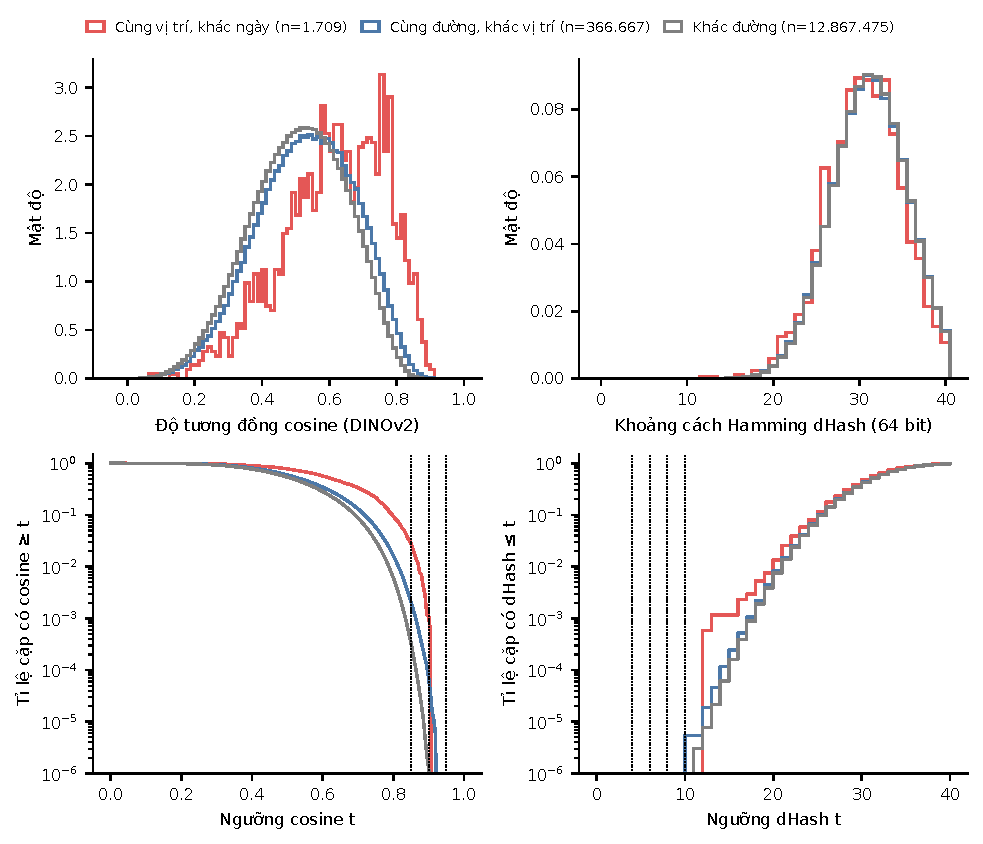
\includegraphics[width=0.92\textwidth]{dup_distance_distributions.pdf}
\caption{Phân bố độ tương đồng giữa các cặp ảnh: cùng vị trí khác ngày, cùng đường khác vị trí, khác đường}
\label{fig:dupdist}
\end{figure}

\subsubsection*{Rò rỉ giữa các tập}

Rò rỉ giữa các tập được đánh giá theo hai cách: theo nội dung ảnh và theo vị trí địa lý (hình~\ref{fig:map}).

\begin{figure}[H]
\centering
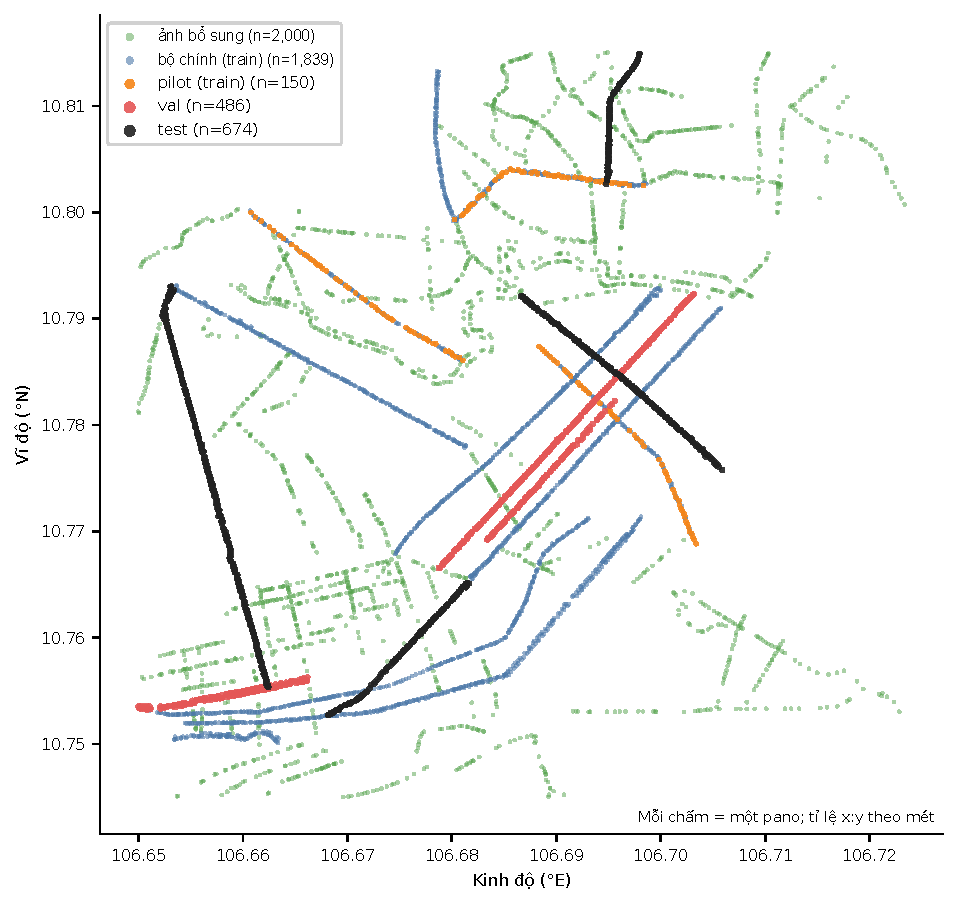
\includegraphics[width=0.8\textwidth]{dup_map_positions.pdf}
\caption{Vị trí của mọi ảnh theo tập. Các đường val/test cắt đường train tại giao lộ}
\label{fig:map}
\end{figure}

\textbf{Theo nội dung ảnh.} Với mỗi ảnh val/test, ảnh giống nhất ở phía train (bộ chính, pilot, ảnh bổ sung) được tìm theo độ tương đồng cosine.
\begin{itemize}
  \item Độ tương đồng với ảnh train gần nhất: val có trung vị 0,78, lớn nhất 0,909; test có trung vị 0,79, lớn nhất 0,904. Phân bố này trùng với mức tham chiếu giữa các đường train với nhau (trung vị 0,81, lớn nhất 0,933); nói cách khác, mức tương đồng giữa val/test và train không cao hơn mức tương đồng giữa hai đường train bất kỳ.
  \item Có 7 ảnh val/test có độ tương đồng cosine $\ge 0{,}90$ với một ảnh train, nhưng cả 7 cặp đều cách nhau 778--3.585 m. Kiểm tra trực quan 20 cặp giống nhau nhất cho thấy đều là hai địa điểm khác nhau có cùng kiểu cảnh (dãy nhà phố, người đi xe máy ở tiền cảnh).
\end{itemize}

\textbf{Theo vị trí địa lý.} Việc chia theo đường không ngăn được trường hợp đường val/test \emph{cắt} đường train tại giao lộ. Bảng~\ref{tab:spatial} thống kê số ảnh val/test nằm gần ảnh phía train.

\begin{table}[H]
\centering
\caption{Số ảnh val/test nằm gần một ảnh phía train}
\label{tab:spatial}
\begin{tabularx}{\textwidth}{>{\raggedright\arraybackslash}p{0.3\linewidth} R R R R R}
\toprule
\textbf{Cặp} & \textbf{Gần nhất (m)} & \textbf{< 15 m} & \textbf{< 25 m} & \textbf{< 40 m} & \textbf{< 100 m} \\
\midrule
Val (486) -- train bộ chính & 1,5 & 6 & 6 & 14 & 47 \\
Val -- pilot & 17,9 & 0 & 1 & 5 & 17 \\
Val -- ảnh bổ sung & 41,6 & 0 & 0 & 0 & 71 \\
Test (674) -- train bộ chính & 7,1 & 8 & 18 & 34 & 88 \\
Test -- pilot & 20,9 & 0 & 2 & 4 & 7 \\
Test -- ảnh bổ sung & 34,3 & 0 & 0 & 3 & 116 \\
\bottomrule
\end{tabularx}
\end{table}

\begin{itemize}
  \item \textbf{52 trên 1.160 ảnh val/test (4,5\%) nằm cách một ảnh train dưới 40 m}, liên quan tới 47 ảnh phía train và 13 cặp đường giao nhau (ví dụ Hồng Bàng -- Nguyễn Trãi, Lý Thường Kiệt -- Cách Mạng Tháng Tám, Hai Bà Trưng -- Điện Biên Phủ).
  \item Kiểm tra trực quan 20 cặp gần nhau nhất (1--14 m): phần lớn nhìn về hai hướng khác nhau, nhưng một số cặp thấy cùng một góc phố (cùng cột điện, biển quảng cáo, hàng rào). Phép đo theo nội dung không phát hiện được các cặp này: độ tương đồng cosine lớn nhất của chúng chỉ là 0,82.
  \item \textbf{Ảnh bổ sung tuân thủ quy tắc 40 m}, trừ 1 ảnh cách ảnh test 34,3 m (do quy tắc được áp dụng cho tâm của ô 25 m, không áp dụng cho từng ảnh).
  \item 53 trên 551 chuỗi ảnh Mapillary chứa ảnh của cả phía train lẫn val/test (cùng một lượt xe chạy qua nhiều đường). Đây không phải rò rỉ nội dung, nhưng cho thấy cùng một thiết bị và điều kiện chụp xuất hiện ở cả hai phía.
\end{itemize}

\textbf{Kế hoạch xử lý} (chưa thực hiện, cần nhóm quyết định trước khi khóa chia tập): loại khỏi train các ảnh cách ảnh val/test dưới 40 m, tương tự quy tắc đã áp dụng cho ảnh bổ sung. Quy tắc này chỉ dùng tọa độ, không dùng nhãn val/test, và loại tối đa 47 ảnh train. Phương án thay thế là giữ nguyên dữ liệu và báo cáo kết quả test kèm một lượt đánh giá loại bỏ 52 ảnh gần giao lộ.

\subsubsection*{Mức khác biệt giữa ảnh bổ sung và bộ chính}

Một bộ phân loại tuyến tính trên vector đặc trưng DINOv2, không dùng nhãn vật cản, được huấn luyện để phân biệt hai nhóm ảnh; AUC bằng 0,5 nghĩa là không phân biệt được. Việc đánh giá dùng xác thực chéo (cross-validation) chia theo đường. Bảng~\ref{tab:domain} trình bày kết quả; hình~\ref{fig:tsne} minh họa phân bố các vector đặc trưng bằng t-SNE.

\begin{figure}[H]
\centering
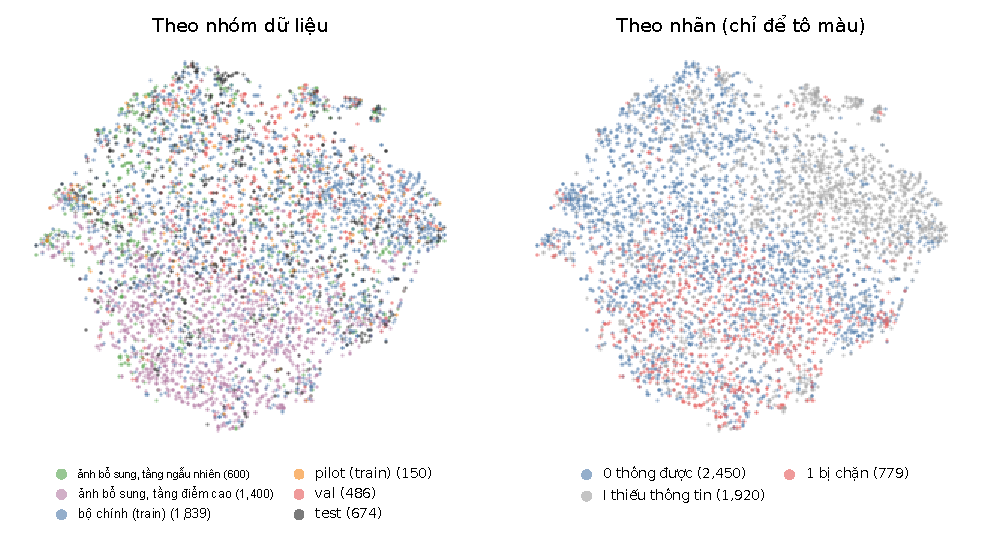
\includegraphics[width=\textwidth]{dup_tsne.pdf}
\caption[Hình chiếu t-SNE của embedding DINOv2 cho 5.149 ảnh, tô theo nhóm và theo nhãn]{Hình chiếu t-SNE~\cite{maaten2008tsne} của embedding DINOv2 cho 5.149 ảnh, tô màu theo nhóm và theo nhãn (nhãn chỉ dùng để tô màu)}
\label{fig:tsne}
\end{figure}

\begin{table}[H]
\centering
\caption{Mức phân biệt được giữa các nhóm ảnh (AUC của bộ phân loại miền)}
\label{tab:domain}
\begin{tabularx}{\textwidth}{>{\raggedright\arraybackslash}p{0.5\linewidth} R L}
\toprule
\textbf{So sánh} & \textbf{AUC} & \textbf{Diễn giải} \\
\midrule
Train bộ chính -- ảnh bổ sung, tầng điểm cao & 0,95 & Khác biệt rõ \\
Train bộ chính -- ảnh bổ sung, tầng ngẫu nhiên & 0,70 & Khác biệt vừa phải \\
Ảnh bổ sung -- val + test & 0,83 & Khác biệt rõ \\
Train bộ chính -- val + test & 0,47 & Không phân biệt được \\
Đối chứng: chia đôi ngẫu nhiên các đường train & 0,51 & Mức nền \\
\bottomrule
\end{tabularx}
\note{Trung bình qua các fold; độ lệch chuẩn giữa các fold 0,02--0,08.}
\end{table}

\begin{itemize}
  \item \textbf{Chưa phát hiện khác biệt miền ảnh giữa train bộ chính và val/test bằng bộ phân loại đã dùng} (AUC gần 0,5); tuy nhiên, kết quả này chưa chứng minh hai phân phối giống nhau. Với chỉ 17 đường, phép đo không đủ nhạy để phát hiện các khác biệt nhỏ.
  \item \textbf{Giá trị gộp 0,47 che khuất các giá trị dao động mạnh khi tách riêng:} train bộ chính so với val là 0,56, so với test là 0,36, so với pilot là 0,35 (trung bình qua các fold; độ lệch chuẩn giữa các fold tới 0,12). AUC dưới 0,5 ở đây không phải tín hiệu ngược chiều mà cho thấy phép đo không ổn định khi mỗi phía chỉ có vài đường.
  \item \textbf{Ảnh bổ sung thuộc một miền khác}, kể cả tầng ngẫu nhiên (0,70): các ảnh này đến từ những đường nhỏ gần chợ, trong khi val/test là các đường lớn. Tầng điểm cao còn đồng nhất hơn các nhóm khác (độ tương đồng cosine trung bình trong nhóm 0,60 so với 0,49--0,51). Đây là sự đánh đổi của việc bổ sung dữ liệu: có thêm 577 mẫu dương nhưng từ một dải cảnh hẹp hơn val/test.
  \item \textbf{Giá trị 0,95 của tầng điểm cao bị ước lượng cao một phần}: tầng này được chọn bằng hồi quy logistic trên chính các vector đặc trưng DINOv2 mà bộ phân loại miền sử dụng, nên một phần khả năng phân biệt đến từ chính cách chọn ảnh. Nhận xét này cũng áp dụng cho độ tương đồng cosine trong nhóm và hình t-SNE. Giá trị phản ánh khách quan hơn mức khác biệt về cảnh là của tầng ngẫu nhiên (0,70).
  \item Trên hình~\ref{fig:tsne}, ảnh \lab{Bị chặn} và ảnh tầng điểm cao tập trung về cùng một vùng, còn ảnh \lab{I} tập trung ở một vùng khác. Hình t-SNE chỉ dùng để minh họa, không dùng để rút ra kết luận.
\end{itemize}

\textbf{Trước khi khóa tập}, nhóm cần quyết định phương án xử lý theo khoảng cách địa lý, lưu manifest với phiên bản cố định và chạy lại các thống kê liên quan. Danh sách đường test được giữ nguyên, không thay đổi dựa trên số mẫu dương đã quan sát.
